%
% fig-paar.tex
%
% (c) 2026 Prof Dr Andreas Müller
%
\begin{figure}
\centering
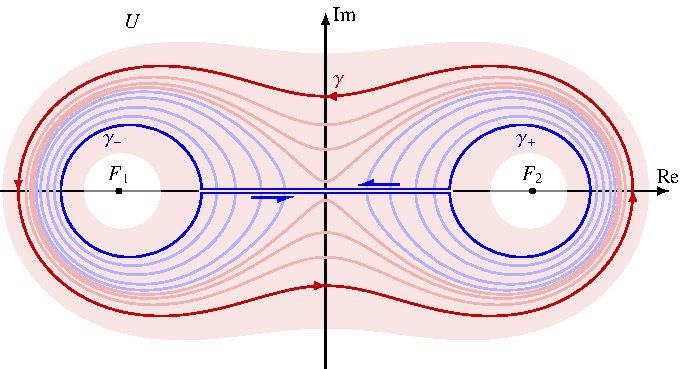
\includegraphics{chapters/030-integration/images/paar.pdf}
\caption{Deformation des Weges $\gamma$ in einen Weg, der die
beiden ``Löcher'' jeweils einmal umlaufen.
Die beiden Wegteile entlang der reellen Achse werden in
entgegengesetzter Richtung durchlaufen, die zugehörigen
Integrale heben sich daher weg.
Der Weg $\gamma$ ist \emph{homolog} zur Summe der Wegen
$\gamma_+$ und $\gamma_-$.
\label{buch:integration:homologie:fig:paar}}
\end{figure}
